Decidimos implementar um Diagrama de Classes pois são diagramas estruturais que permitem ilustrar as classes e o relacionamento entre as mesmas. Assim, estes permitem descrever a estrutura de um sistema, modelando ainda os atributos e as operações entre objetos. \par Nesse sentido, a obtenção deste diagrama resultou de uma análise cuidada do modelo de domínio, identificando assim, quais as classes suscetíveis de serem criadas.

\begin{figure}[H]
\centering
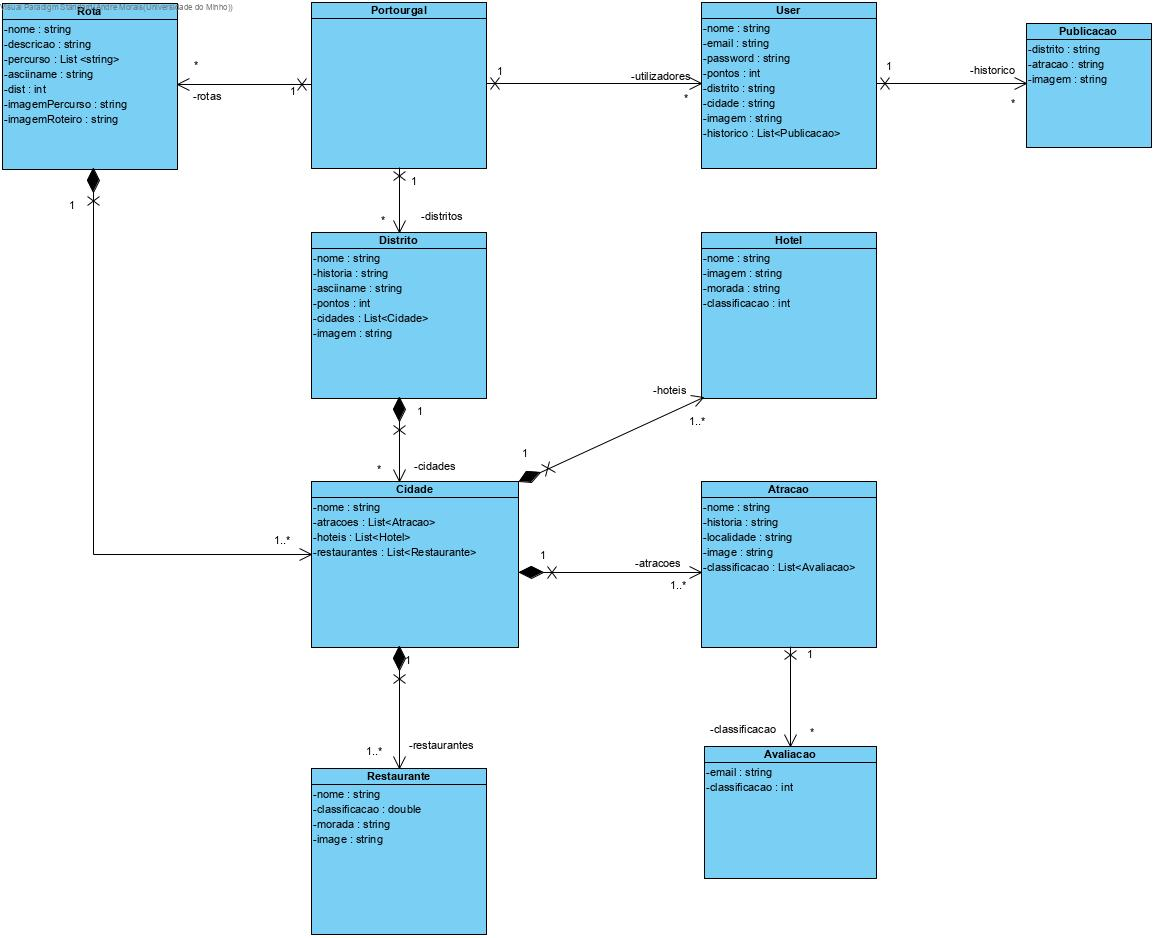
\includegraphics[width=0.9\linewidth]{images/diagrama_classe.jpg}
\caption{Diagrama de classes.}
\end{figure}